% Options for packages loaded elsewhere
\PassOptionsToPackage{unicode}{hyperref}
\PassOptionsToPackage{hyphens}{url}
\PassOptionsToPackage{dvipsnames,svgnames,x11names}{xcolor}
%
\documentclass[
  10pt,
  ignorenonframetext,
  aspectratio=169]{beamer}
\usepackage{pgfpages}
\setbeamertemplate{caption}[numbered]
\setbeamertemplate{caption label separator}{: }
\setbeamercolor{caption name}{fg=normal text.fg}
\beamertemplatenavigationsymbolsempty
% Prevent slide breaks in the middle of a paragraph
\widowpenalties 1 10000
\raggedbottom
\setbeamertemplate{part page}{
  \centering
  \begin{beamercolorbox}[sep=16pt,center]{part title}
    \usebeamerfont{part title}\insertpart\par
  \end{beamercolorbox}
}
\setbeamertemplate{section page}{
  \centering
  \begin{beamercolorbox}[sep=12pt,center]{part title}
    \usebeamerfont{section title}\insertsection\par
  \end{beamercolorbox}
}
\setbeamertemplate{subsection page}{
  \centering
  \begin{beamercolorbox}[sep=8pt,center]{part title}
    \usebeamerfont{subsection title}\insertsubsection\par
  \end{beamercolorbox}
}
\AtBeginPart{
  \frame{\partpage}
}
\AtBeginSection{
  \ifbibliography
  \else
    \frame{\sectionpage}
  \fi
}
\AtBeginSubsection{
  \frame{\subsectionpage}
}
\usepackage{amsmath,amssymb}
\usepackage{lmodern}
\usepackage{iftex}
\ifPDFTeX
  \usepackage[T1]{fontenc}
  \usepackage[utf8]{inputenc}
  \usepackage{textcomp} % provide euro and other symbols
\else % if luatex or xetex
  \usepackage{unicode-math}
  \defaultfontfeatures{Scale=MatchLowercase}
  \defaultfontfeatures[\rmfamily]{Ligatures=TeX,Scale=1}
\fi
\usetheme[]{Singapore}
% Use upquote if available, for straight quotes in verbatim environments
\IfFileExists{upquote.sty}{\usepackage{upquote}}{}
\IfFileExists{microtype.sty}{% use microtype if available
  \usepackage[]{microtype}
  \UseMicrotypeSet[protrusion]{basicmath} % disable protrusion for tt fonts
}{}
\makeatletter
\@ifundefined{KOMAClassName}{% if non-KOMA class
  \IfFileExists{parskip.sty}{%
    \usepackage{parskip}
  }{% else
    \setlength{\parindent}{0pt}
    \setlength{\parskip}{6pt plus 2pt minus 1pt}}
}{% if KOMA class
  \KOMAoptions{parskip=half}}
\makeatother
\usepackage{xcolor}
\newif\ifbibliography
\usepackage{color}
\usepackage{fancyvrb}
\newcommand{\VerbBar}{|}
\newcommand{\VERB}{\Verb[commandchars=\\\{\}]}
\DefineVerbatimEnvironment{Highlighting}{Verbatim}{commandchars=\\\{\}}
% Add ',fontsize=\small' for more characters per line
\usepackage{framed}
\definecolor{shadecolor}{RGB}{48,48,48}
\newenvironment{Shaded}{\begin{snugshade}}{\end{snugshade}}
\newcommand{\AlertTok}[1]{\textcolor[rgb]{1.00,0.81,0.69}{#1}}
\newcommand{\AnnotationTok}[1]{\textcolor[rgb]{0.50,0.62,0.50}{\textbf{#1}}}
\newcommand{\AttributeTok}[1]{\textcolor[rgb]{0.80,0.80,0.80}{#1}}
\newcommand{\BaseNTok}[1]{\textcolor[rgb]{0.86,0.64,0.64}{#1}}
\newcommand{\BuiltInTok}[1]{\textcolor[rgb]{0.80,0.80,0.80}{#1}}
\newcommand{\CharTok}[1]{\textcolor[rgb]{0.86,0.64,0.64}{#1}}
\newcommand{\CommentTok}[1]{\textcolor[rgb]{0.50,0.62,0.50}{#1}}
\newcommand{\CommentVarTok}[1]{\textcolor[rgb]{0.50,0.62,0.50}{\textbf{#1}}}
\newcommand{\ConstantTok}[1]{\textcolor[rgb]{0.86,0.64,0.64}{\textbf{#1}}}
\newcommand{\ControlFlowTok}[1]{\textcolor[rgb]{0.94,0.87,0.69}{#1}}
\newcommand{\DataTypeTok}[1]{\textcolor[rgb]{0.87,0.87,0.75}{#1}}
\newcommand{\DecValTok}[1]{\textcolor[rgb]{0.86,0.86,0.80}{#1}}
\newcommand{\DocumentationTok}[1]{\textcolor[rgb]{0.50,0.62,0.50}{#1}}
\newcommand{\ErrorTok}[1]{\textcolor[rgb]{0.76,0.75,0.62}{#1}}
\newcommand{\ExtensionTok}[1]{\textcolor[rgb]{0.80,0.80,0.80}{#1}}
\newcommand{\FloatTok}[1]{\textcolor[rgb]{0.75,0.75,0.82}{#1}}
\newcommand{\FunctionTok}[1]{\textcolor[rgb]{0.94,0.94,0.56}{#1}}
\newcommand{\ImportTok}[1]{\textcolor[rgb]{0.80,0.80,0.80}{#1}}
\newcommand{\InformationTok}[1]{\textcolor[rgb]{0.50,0.62,0.50}{\textbf{#1}}}
\newcommand{\KeywordTok}[1]{\textcolor[rgb]{0.94,0.87,0.69}{#1}}
\newcommand{\NormalTok}[1]{\textcolor[rgb]{0.80,0.80,0.80}{#1}}
\newcommand{\OperatorTok}[1]{\textcolor[rgb]{0.94,0.94,0.82}{#1}}
\newcommand{\OtherTok}[1]{\textcolor[rgb]{0.94,0.94,0.56}{#1}}
\newcommand{\PreprocessorTok}[1]{\textcolor[rgb]{1.00,0.81,0.69}{\textbf{#1}}}
\newcommand{\RegionMarkerTok}[1]{\textcolor[rgb]{0.80,0.80,0.80}{#1}}
\newcommand{\SpecialCharTok}[1]{\textcolor[rgb]{0.86,0.64,0.64}{#1}}
\newcommand{\SpecialStringTok}[1]{\textcolor[rgb]{0.80,0.58,0.58}{#1}}
\newcommand{\StringTok}[1]{\textcolor[rgb]{0.80,0.58,0.58}{#1}}
\newcommand{\VariableTok}[1]{\textcolor[rgb]{0.80,0.80,0.80}{#1}}
\newcommand{\VerbatimStringTok}[1]{\textcolor[rgb]{0.80,0.58,0.58}{#1}}
\newcommand{\WarningTok}[1]{\textcolor[rgb]{0.50,0.62,0.50}{\textbf{#1}}}
\usepackage{graphicx}
\makeatletter
\def\maxwidth{\ifdim\Gin@nat@width>\linewidth\linewidth\else\Gin@nat@width\fi}
\def\maxheight{\ifdim\Gin@nat@height>\textheight\textheight\else\Gin@nat@height\fi}
\makeatother
% Scale images if necessary, so that they will not overflow the page
% margins by default, and it is still possible to overwrite the defaults
% using explicit options in \includegraphics[width, height, ...]{}
\setkeys{Gin}{width=\maxwidth,height=\maxheight,keepaspectratio}
% Set default figure placement to htbp
\makeatletter
\def\fps@figure{htbp}
\makeatother
\setlength{\emergencystretch}{3em} % prevent overfull lines
\providecommand{\tightlist}{%
  \setlength{\itemsep}{0pt}\setlength{\parskip}{0pt}}
\setcounter{secnumdepth}{-\maxdimen} % remove section numbering
\newenvironment{cols}[1][]{}{}

\newenvironment{col}[1]{\begin{minipage}{#1}\ignorespaces}{%
\end{minipage}
\ifhmode\unskip\fi
\aftergroup\useignorespacesandallpars}

\def\useignorespacesandallpars#1\ignorespaces\fi{%
#1\fi\ignorespacesandallpars}

\makeatletter
\def\ignorespacesandallpars{%
  \@ifnextchar\par
    {\expandafter\ignorespacesandallpars\@gobble}%
    {}%
}
\makeatother
\ifLuaTeX
  \usepackage{selnolig}  % disable illegal ligatures
\fi
\usepackage[]{natbib}
\bibliographystyle{plainnat}
\IfFileExists{bookmark.sty}{\usepackage{bookmark}}{\usepackage{hyperref}}
\IfFileExists{xurl.sty}{\usepackage{xurl}}{} % add URL line breaks if available
\urlstyle{same} % disable monospaced font for URLs
\hypersetup{
  pdftitle={Acquiring and importing texts},
  pdfauthor={Max Callaghan},
  colorlinks=true,
  linkcolor={Maroon},
  filecolor={Maroon},
  citecolor={Blue},
  urlcolor={blue},
  pdfcreator={LaTeX via pandoc}}

\title{Acquiring and importing texts}
\author{Max Callaghan}
\date{2022-09-15}

\begin{document}
\frame{\titlepage}

\hypertarget{objectives}{%
\section{Objectives}\label{objectives}}

\begin{frame}{Methods}
\protect\hypertarget{methods}{}
By the end of this session, you will be able to

\begin{itemize}
  \item<1-> Scrape texts from a website
  \item<2-> Use an API to retrieve texts
  \item<3-> Read texts stored in various formats and process these with R
\end{itemize}
\end{frame}

\begin{frame}{Fundamentals of the internet}
\protect\hypertarget{fundamentals-of-the-internet}{}
You should also acquire some important fundamental knowledge about how
the internet works

\begin{itemize}
  \item<1-> What is a request, how do you make one, and how can this information be specified?
  \item<2-> What responses can be generated from a request, and how can we process these?
  \item<3-> How are html and json files structured, and how can we use them
\end{itemize}
\end{frame}

\begin{frame}{Text sources}
\protect\hypertarget{text-sources}{}
We will explore how to gain access to the following sources of text

\begin{itemize}
  \item<1-> The IEA's Policies and Measures database, by scraping the website
  \item<2-> Scientific articles, using the OpenAlex API
  \item<2-> Twitter posts, using their API
  \item<3-> Parliamentary data, by parsing XML data published by Hansard
\end{itemize}
\end{frame}

\hypertarget{scraping-texts}{%
\section{Scraping texts}\label{scraping-texts}}

\begin{frame}{What does ``scrape'' mean, and why do we need to do it?}
\protect\hypertarget{what-does-scrape-mean-and-why-do-we-need-to-do-it}{}
The internet is full of text data, but it is frequently \emph{presented}
- \textbf{unstructured} - on websites, rather than made available in
\textbf{structured} data files.

If we want to do more than just \textbf{browse} this data, we need to
give our computer instructions on how to systematically download the
data of interest.
\end{frame}

\begin{frame}{What happens when we browse the internet?}
\protect\hypertarget{what-happens-when-we-browse-the-internet}{}
\only<2->{
When we write a url into our web browser and press enter, what we are doing is sending a \textbf{request} to an \textbf{address}.

In our first example, we are going to look at \url{https://www.iea.org/policies}. 

\begin{itemize}
  \item \url{https} defines the \href{https://en.wikipedia.org/wiki/HTTPS}{protocol}
  \item \url{www.iea.org} defines the \href{https://en.wikipedia.org/wiki/Hostname}{hostname}
  \item \url{policies} defines the path on the host containing the resources we require
\end{itemize}

}

\only<3->{
If we click on open the url with chrome or firefox, we can investigate further by opening developer tools (ctrl+shift+i). Today we will look at the \textbf{Network} and \textbf{Elements} tabs
}
\end{frame}

\begin{frame}{Making Requests}
\protect\hypertarget{making-requests}{}
\begin{cols}

\begin{col}{0.35\textwidth}
If you click on the \textbf{Network} tab and refresh, you can see all
the communication that is happening when we visit a page.

Clicking on policies, we can inspect how this starts.

Our browser sends a request to the url, along with \textbf{headers},
which explain how the request should be processed.

We then receive a response, which has content, a status code, and it's
own set of headers.

\end{col}

\begin{col}{0.05\textwidth}
~

\end{col}

\begin{col}{0.60\textwidth}
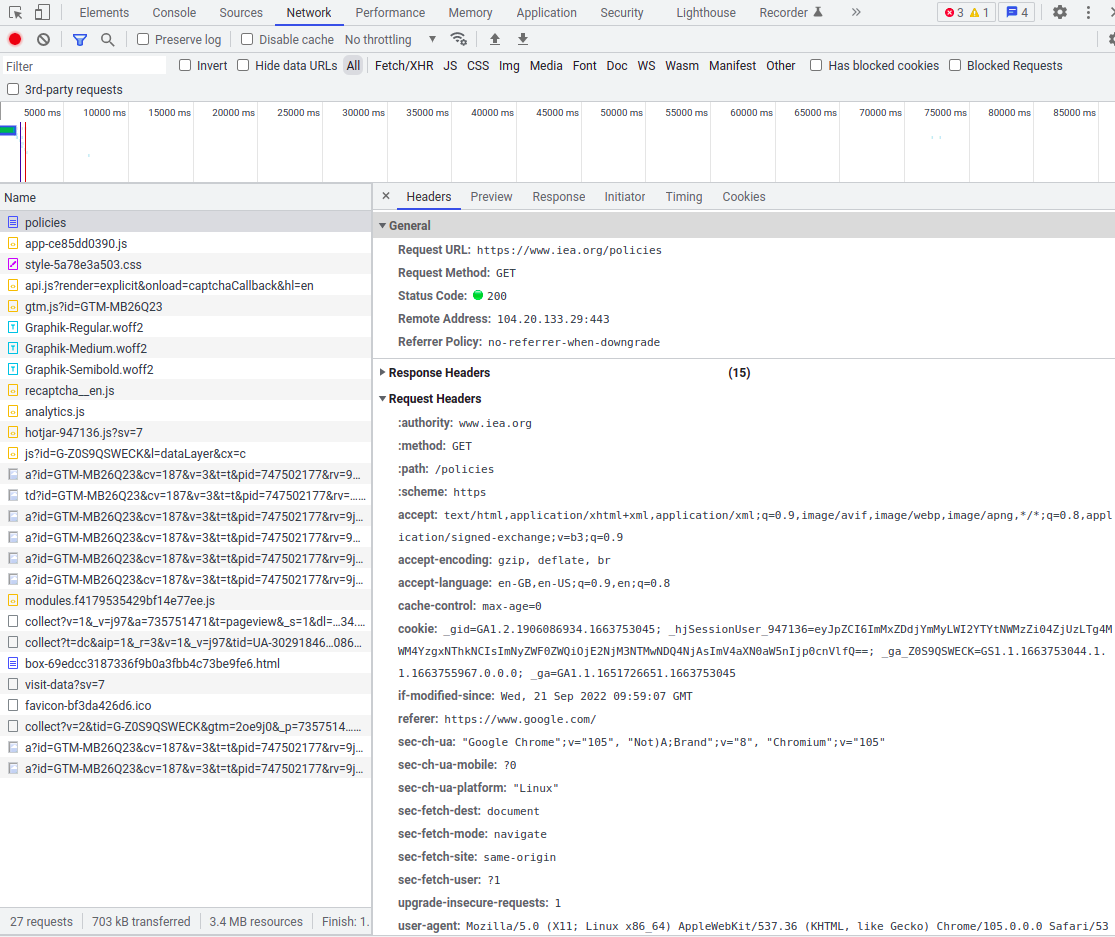
\includegraphics{iea_network_request.png}

\end{col}

\end{cols}
\end{frame}

\begin{frame}[fragile]{Making requests with R}
\protect\hypertarget{making-requests-with-r}{}
We can mimic this R using
\href{https://cran.r-project.org/web/packages/httr/vignettes/quickstart.html}{httr}

\scriptsize

\begin{Shaded}
\begin{Highlighting}[]
\FunctionTok{library}\NormalTok{(httr)}
\NormalTok{r }\OtherTok{\textless{}{-}} \FunctionTok{GET}\NormalTok{(}\StringTok{"https://www.iea.org/policies"}\NormalTok{)}
\NormalTok{r}
\end{Highlighting}
\end{Shaded}

\begin{verbatim}
## Response [https://www.iea.org/policies]
##   Date: 2022-09-21 20:08
##   Status: 200
##   Content-Type: text/html; charset=UTF-8
##   Size: 304 kB
## <!DOCTYPE html>
## <html dir="ltr" lang="en-GB"
##       class="no-js page-all-policies ">
## <head>
##     <meta charset="utf-8">
##     <meta name="viewport" content="width=device-width, initial-scale=1.0">
##     <meta http-equiv="X-UA-Compatible" content="IE=Edge">
##     <meta name="csrf-token" content="">
##     
##     <link rel="shortcut icon" href="/assets/front/images/favicon-bf3da426d6.i...
## ...
\end{verbatim}
\end{frame}

\begin{frame}[fragile]{Making requests with Python}
\protect\hypertarget{making-requests-with-python}{}
In Python, a similar no-frills option is
\href{https://requests.readthedocs.io/en/latest/user/quickstart/}{requests}

\scriptsize

\begin{Shaded}
\begin{Highlighting}[]
\ImportTok{import}\NormalTok{ requests}
\ImportTok{from}\NormalTok{ rich.pretty }\ImportTok{import}\NormalTok{ pprint}
\CommentTok{\#r = requests.get("https://www.iea.org/policies")}
\CommentTok{\#pprint(r.\_\_dict\_\_, max\_string=40)}
\end{Highlighting}
\end{Shaded}
\end{frame}

\begin{frame}[fragile]{Understanding HTML responses}
\protect\hypertarget{understanding-html-responses}{}
\begin{cols}

\begin{col}{0.35\textwidth}

If you click on the \textbf{Elements} tab, you will see the HTML
response of the website.

~

HTML is a hierarchical structure of
\href{https://developer.mozilla.org/en-US/docs/Web/HTML/Element}{elements}
\texttt{\textless{}p\textgreater{}Hello\textless{}/p\textgreater{}}. In
this hierarchy we refer to

\begin{itemize}
\tightlist
\item
  the \textbf{root}
\item
  parents
\item
  children
\item
  siblings
\end{itemize}

\end{col}

\begin{col}{0.05\textwidth}
~

\end{col}

\begin{col}{0.60\textwidth}
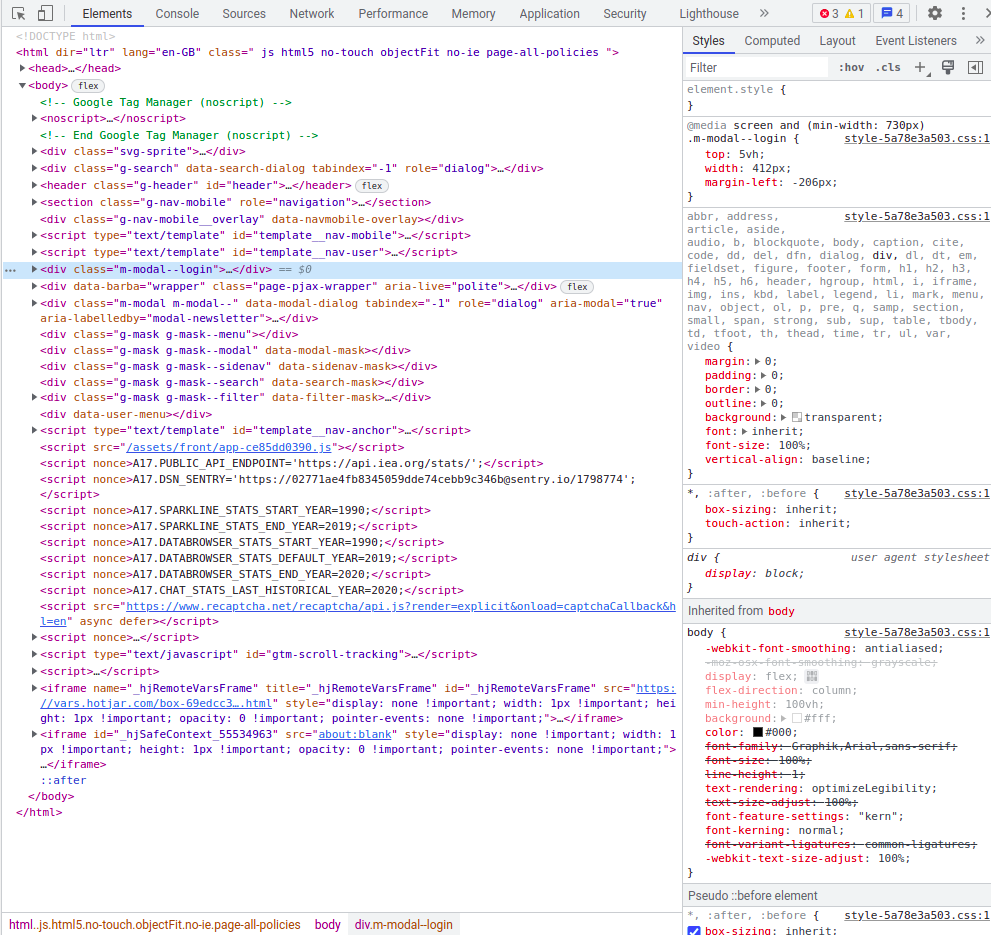
\includegraphics{iea_html.png}

\end{col}

\end{cols}
\end{frame}

\begin{frame}[fragile]{What is in a web element?}
\protect\hypertarget{what-is-in-a-web-element}{}
The element \textbf{name} is the first word after the opening
\texttt{\textless{}}, and describes what \emph{type} of element it is.

The element's \textbf{attributes} are the key, value pairs either side
of the \texttt{=} signs before the \texttt{\textgreater{}}.

Element's should be closed with a \texttt{/} and a
\texttt{\textgreater{}}.
\texttt{\textless{}a\textgreater{}\textless{}/a\textgreater{}} and
\texttt{\textless{}a/\textgreater{}} are both closed.

Anything between opening and closing tags
(\texttt{\textless{}\textgreater{}}) is the element's content, or inner
html. It can contain further elements (children)

You can find an element by clicking on the icon with the cursor in the
developer tools

\begin{verbatim}
<a class="m-policy-listing-item__link" 
href="/policies/12654-emissions-limit-on-the-capacity-market-regulations">
Emissions limit on the Capacity Market Regulations
</a>
\end{verbatim}
\end{frame}

\begin{frame}[fragile]{Scraping elements}
\protect\hypertarget{scraping-elements}{}
In our example from the IEA, we want to identify each element linking to
a policy, and find a common feature of those links. We can select these
by passing
\href{https://developer.mozilla.org/en-US/docs/Learn/CSS/Building_blocks/Selectors}{css
selectors} to the \texttt{html\_elements} function from
\href{https://rvest.tidyverse.org/}{rvest}

In this case they all have the class ``m-policy-listing-item\_\_link''

\scriptsize

\begin{Shaded}
\begin{Highlighting}[]
\FunctionTok{library}\NormalTok{(rvest)}
\NormalTok{html }\OtherTok{\textless{}{-}} \FunctionTok{read\_html}\NormalTok{(}\StringTok{"https://www.iea.org/policies"}\NormalTok{)}
\NormalTok{links }\OtherTok{\textless{}{-}}\NormalTok{ html }\SpecialCharTok{\%\textgreater{}\%} \FunctionTok{html\_elements}\NormalTok{(}\StringTok{"a.m{-}policy{-}listing{-}item\_\_link"}\NormalTok{)}
\NormalTok{links}
\end{Highlighting}
\end{Shaded}

\begin{verbatim}
## {xml_nodeset (30)}
##  [1] <a class="m-policy-listing-item__link" href="/policies/11663-fuel-econom ...
##  [2] <a class="m-policy-listing-item__link" href="/policies/12654-emissions-l ...
##  [3] <a class="m-policy-listing-item__link" href="/policies/8506-gas-boilers- ...
##  [4] <a class="m-policy-listing-item__link" href="/policies/3124-local-govern ...
##  [5] <a class="m-policy-listing-item__link" href="/policies/12046-decommissio ...
##  [6] <a class="m-policy-listing-item__link" href="/policies/8401-enhancements ...
##  [7] <a class="m-policy-listing-item__link" href="/policies/12197-heavy-goods ...
##  [8] <a class="m-policy-listing-item__link" href="/policies/11497-proposals-f ...
##  [9] <a class="m-policy-listing-item__link" href="/policies/13139-resolution- ...
## [10] <a class="m-policy-listing-item__link" href="/policies/11456-updated-mep ...
## [11] <a class="m-policy-listing-item__link" href="/policies/15028-france-2030 ...
## [12] <a class="m-policy-listing-item__link" href="/policies/15026-france-2030 ...
## [13] <a class="m-policy-listing-item__link" href="/policies/15025-france-2030 ...
## [14] <a class="m-policy-listing-item__link" href="/policies/14279-france-2030 ...
## [15] <a class="m-policy-listing-item__link" href="/policies/15029-france-2030 ...
## [16] <a class="m-policy-listing-item__link" href="/policies/14465-france-2030 ...
## [17] <a class="m-policy-listing-item__link" href="/policies/15027-france-2030 ...
## [18] <a class="m-policy-listing-item__link" href="/policies/15780-inner-mongo ...
## [19] <a class="m-policy-listing-item__link" href="/policies/13751-2022-eu-bud ...
## [20] <a class="m-policy-listing-item__link" href="/policies/13231-2022-2033-n ...
## ...
\end{verbatim}
\end{frame}

\begin{frame}[fragile]{Scraping elements}
\protect\hypertarget{scraping-elements-1}{}
In our example from the IEA, we want to identify each element linking to
a policy, and find a common feature of those links. We can select these
by passing
\href{https://developer.mozilla.org/en-US/docs/Learn/CSS/Building_blocks/Selectors}{css
selectors} to the \texttt{select} function of
\href{https://www.crummy.com/software/BeautifulSoup/bs4/doc/\#css-selectors}{Beautiful
Soup}

In this case they all have the class ``m-policy-listing-item\_\_link''

\scriptsize

\begin{Shaded}
\begin{Highlighting}[]
\ImportTok{import}\NormalTok{ requests}
\ImportTok{from}\NormalTok{ bs4 }\ImportTok{import}\NormalTok{ BeautifulSoup}
\NormalTok{r }\OperatorTok{=}\NormalTok{ requests.get(}\StringTok{"https://www.iea.org/policies"}\NormalTok{)}
\NormalTok{soup }\OperatorTok{=}\NormalTok{ BeautifulSoup(r.content)}
\NormalTok{links }\OperatorTok{=}\NormalTok{ soup.select(}\StringTok{"a.m{-}policy{-}listing{-}item\_\_link"}\NormalTok{)}
\NormalTok{links}
\end{Highlighting}
\end{Shaded}

\begin{verbatim}
## [<a class="m-policy-listing-item__link" href="/policies/11663-fuel-economy-standards-on-light-duty-vehicles">Fuel Economy Standards on Light-Duty Vehicles
##                                                     </a>, <a class="m-policy-listing-item__link" href="/policies/12654-emissions-limit-on-the-capacity-market-regulations">Emissions limit on the Capacity Market Regulations
##                                                     </a>, <a class="m-policy-listing-item__link" href="/policies/8506-gas-boilers-replacement-by-low-carbon-heating-systems">Gas boilers replacement by low-carbon heating systems
##                                                     </a>, <a class="m-policy-listing-item__link" href="/policies/3124-local-government-fleet-renewal-mandate">Local Government fleet renewal mandate
##                                                     </a>, <a class="m-policy-listing-item__link" href="/policies/12046-decommissioning-fossil-fuel-power-plants">Decommissioning fossil fuel power plants
##                                                     </a>, <a class="m-policy-listing-item__link" href="/policies/8401-enhancements-to-minimum-energy-performance-standards-meps">Enhancements to Minimum Energy Performance Standards (MEPS)
##                                                     </a>, <a class="m-policy-listing-item__link" href="/policies/12197-heavy-goods-vehicle-charge">Heavy goods vehicle charge
##                                                     </a>, <a class="m-policy-listing-item__link" href="/policies/11497-proposals-for-location-of-wind-power-turbines">Proposals for location of wind power turbines
##                                                     </a>, <a class="m-policy-listing-item__link" href="/policies/13139-resolution-407152019-wholesale-energy-market-with-res-in-2023">Resolution 40715/2019: Wholesale Energy Market with RES in 2023
##                                                     </a>, <a class="m-policy-listing-item__link" href="/policies/11456-updated-meps-central-air-conditioners-and-heat-pumps">Updated MEPS - Central Air Conditioners and Heat Pumps
##                                                     </a>, <a class="m-policy-listing-item__link" href="/policies/15028-france-2030-investment-plan-small-modular-reactor-investment">"France 2030 Investment Plan"- Small Modular Reactor investment
##                                                     </a>, <a class="m-policy-listing-item__link" href="/policies/15026-france-2030-investment-plan-critical-minerals-investment">"France 2030 investment Plan"- Critical minerals investment
##                                                     </a>, <a class="m-policy-listing-item__link" href="/policies/15025-france-2030-investment-plan-investment-in-renewable-energy-innovation">"France 2030 investment Plan"- Investment in renewable energy innovation 
##                                                     </a>, <a class="m-policy-listing-item__link" href="/policies/14279-france-2030-investment-plan">"France 2030" Investment Plan
##                                                     </a>, <a class="m-policy-listing-item__link" href="/policies/15029-france-2030-investment-plan-heavy-industry-decarbonisation-investment">"France 2030" Investment Plan- Heavy industry decarbonisation investment
##                                                     </a>, <a class="m-policy-listing-item__link" href="/policies/14465-france-2030-investment-plan-hydrogen-sector-funding">"France 2030" Investment Plan- Hydrogen sector funding
##                                                     </a>, <a class="m-policy-listing-item__link" href="/policies/15027-france-2030-investment-plan-clean-transport-investment">"France 2030" investment plan- Clean transport investment
##                                                     </a>, <a class="m-policy-listing-item__link" href="/policies/15780-inner-mongolia-coal-industry-development-14th-five-year-plan-coalbed-methane-development-and-utilization-supporting-scheme">(Inner Mongolia) Coal Industry Development 14th Five-Year Plan - Coalbed Methane Development and Utilization Supporting Scheme
##                                                     </a>, <a class="m-policy-listing-item__link" href="/policies/13751-2022-eu-budget">2022  EU budget
##                                                     </a>, <a class="m-policy-listing-item__link" href="/policies/13231-2022-2033-national-transport-plan-railway">2022 - 2033 National Transport Plan - Railway
##                                                     </a>, <a class="m-policy-listing-item__link" href="/policies/13238-2022-2033-national-transport-plan-urban-growth-agreement">2022 - 2033 National Transport Plan - Urban growth agreement
##                                                     </a>, <a class="m-policy-listing-item__link" href="/policies/13239-2022-2033-national-transport-plan-water-transport">2022 - 2033 National Transport Plan - Water transport
##                                                     </a>, <a class="m-policy-listing-item__link" href="/policies/13240-2022-2033-national-transport-plan-new-airports">2022 -2033 National Transport Plan - New airports
##                                                     </a>, <a class="m-policy-listing-item__link" href="/policies/14813-2022-round-of-subsidies-for-e-mobility">2022 round of subsidies for e-mobility
##                                                     </a>, <a class="m-policy-listing-item__link" href="/policies/14885-aud-7-million-grants-on-hydrogen-fuelled-cremations-fuel-cell-buses">AUD 7 million grants on hydrogen fuelled cremations, fuel cell buses
##                                                     </a>, <a class="m-policy-listing-item__link" href="/policies/14890-aid-for-municipal-infrastructure-for-just-transition">Aid for municipal infrastructure for Just Transition
##                                                     </a>, <a class="m-policy-listing-item__link" href="/policies/14499-budget-agreement-2022-green-initiatives-and-sustainable-energy-portfolio">Budget Agreement 2022: Green Initiatives and Sustainable Energy Portfolio
##                                                     </a>, <a class="m-policy-listing-item__link" href="/policies/15589-california-governors-budget-summary-lithium-valley-development">California Governor's Budget Summary: Lithium Valley Development
##                                                     </a>, <a class="m-policy-listing-item__link" href="/policies/14212-carbon-neutrality-and-green-growth-act-for-the-climate-change">Carbon Neutrality and Green Growth Act for the Climate Change
##                                                     </a>, <a class="m-policy-listing-item__link" href="/policies/11685-clean-fuel-standard">Clean Fuel Standard
##                                                     </a>]
\end{verbatim}
\end{frame}

\begin{frame}[fragile]{Following links and extracting information}
\protect\hypertarget{following-links-and-extracting-information}{}
Now we want to follow each of these links, parse the website, and
extract the information we want

\scriptsize

\begin{Shaded}
\begin{Highlighting}[]
\FunctionTok{library}\NormalTok{(tibble)}
\NormalTok{df }\OtherTok{\textless{}{-}} \FunctionTok{tibble}\NormalTok{(}\AttributeTok{text=}\FunctionTok{character}\NormalTok{())}
\ControlFlowTok{for}\NormalTok{ (link }\ControlFlowTok{in} \FunctionTok{html\_attr}\NormalTok{(links,}\StringTok{"href"}\NormalTok{)) \{}
\NormalTok{  link\_html }\OtherTok{\textless{}{-}} \FunctionTok{read\_html}\NormalTok{(}\FunctionTok{paste0}\NormalTok{(}\StringTok{"https://iea.org"}\NormalTok{,link))}
\NormalTok{  text }\OtherTok{\textless{}{-}}\NormalTok{ link\_html }\SpecialCharTok{\%\textgreater{}\%} \FunctionTok{html\_element}\NormalTok{(}\StringTok{"div.m{-}block p"}\NormalTok{) }\SpecialCharTok{\%\textgreater{}\%} \FunctionTok{html\_text}\NormalTok{()}
\NormalTok{  df }\OtherTok{\textless{}{-}}\NormalTok{ df }\SpecialCharTok{\%\textgreater{}\%} \FunctionTok{add\_row}\NormalTok{(}\AttributeTok{text=}\NormalTok{text)}
  \ControlFlowTok{break}
\NormalTok{\}}
\NormalTok{df}
\end{Highlighting}
\end{Shaded}

\begin{verbatim}
## # A tibble: 1 x 1
##   text                                                                          
##   <chr>                                                                         
## 1 Japan sets and periodically updates fuel economy standards on cars, vans and ~
\end{verbatim}
\end{frame}

\begin{frame}[fragile]{Following links and extracting information}
\protect\hypertarget{following-links-and-extracting-information-1}{}
Now we want to follow each of these links, parse the html, and extract
the information we want

\scriptsize

\begin{Shaded}
\begin{Highlighting}[]
\ImportTok{import}\NormalTok{ pandas }\ImportTok{as}\NormalTok{ pd}
\NormalTok{data }\OperatorTok{=}\NormalTok{ []}
\ControlFlowTok{for}\NormalTok{ link }\KeywordTok{in}\NormalTok{ links:}
\NormalTok{    r }\OperatorTok{=}\NormalTok{ requests.get(}\StringTok{"https://iea.org"} \OperatorTok{+}\NormalTok{ link[}\StringTok{"href"}\NormalTok{])}
\NormalTok{    link\_soup }\OperatorTok{=}\NormalTok{ BeautifulSoup(r.content)}
\NormalTok{    data.append(\{}\StringTok{"text"}\NormalTok{: link\_soup.select(}\StringTok{"div.m{-}block p"}\NormalTok{)[}\DecValTok{0}\NormalTok{].text\})}
    \ControlFlowTok{break}
    
\NormalTok{df }\OperatorTok{=}\NormalTok{ pd.DataFrame.from\_dict(data)}
\NormalTok{df}
\end{Highlighting}
\end{Shaded}

\begin{verbatim}
##                                                 text
## 0  Japan sets and periodically updates fuel econo...
\end{verbatim}
\end{frame}

\begin{frame}{Exercise}
\protect\hypertarget{exercise}{}
Now in pairs, build a scraper that returns a dataframe with the columns
{[}Country, Year, Status, Jurisdiction, Text, Link, Topics, Policy
types, Sectors, Technologies{]}

How would you extend this scraper to collect the whole database (not
just the first page)?
\end{frame}

\hypertarget{apis}{%
\section{APIs}\label{apis}}

\begin{frame}{What is an API and how do I use it?}
\protect\hypertarget{what-is-an-api-and-how-do-i-use-it}{}
An API is a \emph{predefined} set of possible requests, with a given set
of possible responses and response formats.

APIs usually return \textbf{data} rather than instructions for building
a web page.

They are explicitly built for access by machines, and should stay
consistent over time.

\medskip

\only<2->{

The first API we will look at is for the open catalog of scientific research \href{https://docs.openalex.org/}{OpenAlex}

For more details on OpenAlex, have a look at this \href{https://github.com/mcallaghan/NLP-climate-science-tutorial-CCAI/blob/main/A_obtaining_data.ipynb}{tutorial} I gave for a summer school.

}
\end{frame}

\begin{frame}{Constructing an API call}
\protect\hypertarget{constructing-an-api-call}{}
Let's start by searching the institutions endpoint for the Hertie School

\url{https://api.openalex.org/institutions?filter=display_name.search:hertie}

We can plug the ID we find here into a query of the works enpoint, where
we search works where an author is affiliated with Hertie

\url{https://api.openalex.org/works?filter=authorships.institutions.id:I24830596}
\end{frame}

\begin{frame}[fragile]{Parsing Json}
\protect\hypertarget{parsing-json}{}
Now we just need to parse the json, which is very easy in python

\scriptsize

\begin{Shaded}
\begin{Highlighting}[]
\ImportTok{from}\NormalTok{ dotenv }\ImportTok{import}\NormalTok{ load\_dotenv}
\ImportTok{import}\NormalTok{ os}
\NormalTok{load\_dotenv()}
\end{Highlighting}
\end{Shaded}

\begin{verbatim}
## True
\end{verbatim}

\begin{Shaded}
\begin{Highlighting}[]
\NormalTok{headers }\OperatorTok{=}\NormalTok{ \{}\StringTok{"email"}\NormalTok{: os.getenv(}\StringTok{"email"}\NormalTok{)\}}
\NormalTok{r }\OperatorTok{=}\NormalTok{ requests.get(}
  \StringTok{"https://api.openalex.org/works?filter=authorships.institutions.id:I24830596"}\NormalTok{,}
\NormalTok{  headers}\OperatorTok{=}\NormalTok{headers}
\NormalTok{)}
\NormalTok{res }\OperatorTok{=}\NormalTok{ r.json()}
\NormalTok{pprint(res, max\_string}\OperatorTok{=}\DecValTok{21}\NormalTok{, max\_length}\OperatorTok{=}\DecValTok{5}\NormalTok{)}
\end{Highlighting}
\end{Shaded}

\begin{verbatim}
## {
## │   'meta': {
## │   │   'count': 1275,
## │   │   'db_response_time_ms': 46,
## │   │   'page': 1,
## │   │   'per_page': 25
## │   },
## │   'results': [
## │   │   {
## │   │   │   'id': 'https://openalex.org/'+11,
## │   │   │   'doi': 'https://doi.org/10.10'+15,
## │   │   │   'title': 'Biophysical and econo'+36,
## │   │   │   'display_name': 'Biophysical and econo'+36,
## │   │   │   'publication_year': 2016,
## │   │   │   ... +21
## │   │   },
## │   │   {
## │   │   │   'id': 'https://openalex.org/'+9,
## │   │   │   'doi': 'https://doi.org/10.10'+23,
## │   │   │   'title': 'New Social Movements:'+60,
## │   │   │   'display_name': 'New Social Movements:'+60,
## │   │   │   'publication_year': 2019,
## │   │   │   ... +21
## │   │   },
## │   │   {
## │   │   │   'id': 'https://openalex.org/'+11,
## │   │   │   'doi': 'https://doi.org/10.11'+18,
## │   │   │   'title': 'From Intergovernmenta'+89,
## │   │   │   'display_name': 'From Intergovernmenta'+89,
## │   │   │   'publication_year': 1997,
## │   │   │   ... +21
## │   │   },
## │   │   {
## │   │   │   'id': 'https://openalex.org/'+11,
## │   │   │   'doi': 'https://doi.org/10.10'+21,
## │   │   │   'title': 'The governance of soc'+84,
## │   │   │   'display_name': 'The governance of soc'+84,
## │   │   │   'publication_year': 2014,
## │   │   │   ... +21
## │   │   },
## │   │   {
## │   │   │   'id': 'https://openalex.org/'+11,
## │   │   │   'doi': 'https://doi.org/10.10'+20,
## │   │   │   'title': 'Organizing for Societ'+46,
## │   │   │   'display_name': 'Organizing for Societ'+46,
## │   │   │   'publication_year': 2012,
## │   │   │   ... +21
## │   │   },
## │   │   ... +20
## │   ],
## │   'group_by': []
## }
\end{verbatim}
\end{frame}

\begin{frame}[fragile]{Parsing Json}
\protect\hypertarget{parsing-json-1}{}
Now we just need to parse the json, which is very easy in python, and a
bit of a pain in R. For now we'll just let create a dataframe with
dataframes inside it

\scriptsize

\begin{Shaded}
\begin{Highlighting}[]
\FunctionTok{library}\NormalTok{(jsonlite)}
\FunctionTok{library}\NormalTok{(dplyr)}
\FunctionTok{library}\NormalTok{(dotenv)}
\FunctionTok{load\_dot\_env}\NormalTok{(}\StringTok{".env"}\NormalTok{)}
\NormalTok{r }\OtherTok{\textless{}{-}} \FunctionTok{GET}\NormalTok{(}
  \StringTok{"https://api.openalex.org/works?filter=authorships.institutions.id:I24830596"}\NormalTok{,}
  \FunctionTok{add\_headers}\NormalTok{(}\AttributeTok{email=}\FunctionTok{Sys.getenv}\NormalTok{(}\StringTok{"email"}\NormalTok{))}
\NormalTok{  )}
\NormalTok{data }\OtherTok{\textless{}{-}} \FunctionTok{fromJSON}\NormalTok{(}\FunctionTok{content}\NormalTok{(r, }\StringTok{"text"}\NormalTok{))}
\end{Highlighting}
\end{Shaded}

\begin{verbatim}
## No encoding supplied: defaulting to UTF-8.
\end{verbatim}

\begin{Shaded}
\begin{Highlighting}[]
\NormalTok{df }\OtherTok{\textless{}{-}} \FunctionTok{cbind}\NormalTok{(}
  \FunctionTok{select}\NormalTok{(data}\SpecialCharTok{$}\NormalTok{results, }\FunctionTok{where}\NormalTok{(is.character)), }
  \FunctionTok{select}\NormalTok{(data}\SpecialCharTok{$}\NormalTok{results, }\FunctionTok{where}\NormalTok{(is.numeric))}
\NormalTok{)}
\FunctionTok{head}\NormalTok{(df)}
\end{Highlighting}
\end{Shaded}

\begin{verbatim}
##                                 id                                          doi
## 1 https://openalex.org/W2195453830         https://doi.org/10.1038/nclimate2870
## 2   https://openalex.org/W18536190 https://doi.org/10.1007/978-3-658-22261-1_12
## 3 https://openalex.org/W2041842081      https://doi.org/10.1111/1468-0386.00031
## 4 https://openalex.org/W2092902022   https://doi.org/10.1016/j.riob.2014.09.001
## 5 https://openalex.org/W2003457148    https://doi.org/10.1007/s10551-012-1414-3
## 6 https://openalex.org/W1483436082     https://doi.org/10.1177/0170840615580007
##                                                                                                            title
## 1                                                      Biophysical and economic limits to negative CO2 emissions
## 2                              New Social Movements: Challenging the Boundaries of Institutional Politics (1985)
## 3 From Intergovernmental Bargaining to Deliberative Political Processes: The Constitutionalisation of Comitology
## 4      The governance of social enterprises: Mission drift and accountability challenges in hybrid organizations
## 5                                            Organizing for Society: A Typology of Social Entrepreneuring Models
## 6                          Navigating Institutional Plurality: Organizational Governance in Hybrid Organizations
##                                                                                                     display_name
## 1                                                      Biophysical and economic limits to negative CO2 emissions
## 2                              New Social Movements: Challenging the Boundaries of Institutional Politics (1985)
## 3 From Intergovernmental Bargaining to Deliberative Political Processes: The Constitutionalisation of Comitology
## 4      The governance of social enterprises: Mission drift and accountability challenges in hybrid organizations
## 5                                            Organizing for Society: A Typology of Social Entrepreneuring Models
## 6                          Navigating Institutional Plurality: Organizational Governance in Hybrid Organizations
##   publication_date            type
## 1       2016-01-01 journal-article
## 2       2019-01-01    book-chapter
## 3       1997-09-01 journal-article
## 4       2014-01-01 journal-article
## 5       2012-08-01 journal-article
## 6       2015-06-01 journal-article
##                                          ngrams_url
## 1 https://api.openalex.org/works/W2195453830/ngrams
## 2   https://api.openalex.org/works/W18536190/ngrams
## 3 https://api.openalex.org/works/W2041842081/ngrams
## 4 https://api.openalex.org/works/W2092902022/ngrams
## 5 https://api.openalex.org/works/W2003457148/ngrams
## 6 https://api.openalex.org/works/W1483436082/ngrams
##                                          cited_by_api_url
## 1 https://api.openalex.org/works?filter=cites:W2195453830
## 2   https://api.openalex.org/works?filter=cites:W18536190
## 3 https://api.openalex.org/works?filter=cites:W2041842081
## 4 https://api.openalex.org/works?filter=cites:W2092902022
## 5 https://api.openalex.org/works?filter=cites:W2003457148
## 6 https://api.openalex.org/works?filter=cites:W1483436082
##                 updated_date created_date publication_year cited_by_count
## 1 2022-09-20T01:27:30.114154   2016-06-24             2016            704
## 2 2022-09-18T11:18:23.407584   2016-06-24             2019            565
## 3 2022-09-15T19:58:30.845548   2016-06-24             1997            508
## 4 2022-09-21T15:38:48.322246   2016-06-24             2014            500
## 5 2022-09-06T23:52:55.318454   2016-06-24             2012            282
## 6 2022-09-20T16:12:18.762653   2016-06-24             2015            232
\end{verbatim}
\end{frame}

\begin{frame}{Paginated results}
\protect\hypertarget{paginated-results}{}
Where datasets are large, APIs will often not give us the whole dataset
at once, but deliver it in chunks. They will have their own way of
letting us navigate through these, but often this will involve cursors.

With open Alex, we simply add \url{&cursor=*} to our url the first time
we make a request, and keep using the new cursor it returns until it is
Null
\end{frame}

\begin{frame}[fragile]{Paginated results}
\protect\hypertarget{paginated-results-1}{}
\scriptsize

\begin{Shaded}
\begin{Highlighting}[]
\NormalTok{cursor }\OtherTok{\textless{}{-}} \StringTok{"*"}
\NormalTok{base\_url }\OtherTok{\textless{}{-}} \StringTok{"https://api.openalex.org/works?filter=authorships.institutions.id:I24830596"}
\NormalTok{df }\OtherTok{\textless{}{-}} \ConstantTok{NULL}
\ControlFlowTok{while}\NormalTok{ (}\SpecialCharTok{!}\FunctionTok{is.null}\NormalTok{(cursor)) \{}
\NormalTok{  r }\OtherTok{\textless{}{-}} \FunctionTok{GET}\NormalTok{(}\FunctionTok{paste0}\NormalTok{(}
\NormalTok{    base\_url, }\StringTok{"\&per{-}page=200"}\NormalTok{,}
    \StringTok{"\&cursor="}\NormalTok{,cursor}
\NormalTok{  ), }\FunctionTok{add\_headers}\NormalTok{(}\AttributeTok{email=}\FunctionTok{Sys.getenv}\NormalTok{(}\StringTok{"email"}\NormalTok{)))}
\NormalTok{  data }\OtherTok{\textless{}{-}} \FunctionTok{fromJSON}\NormalTok{(}\FunctionTok{content}\NormalTok{(r, }\StringTok{"text"}\NormalTok{, }\AttributeTok{encoding=}\StringTok{"utf{-}8"}\NormalTok{), }\AttributeTok{simplifyDataFrame =} \ConstantTok{TRUE}\NormalTok{)}
  \ControlFlowTok{if}\NormalTok{ (}\FunctionTok{length}\NormalTok{(data}\SpecialCharTok{$}\NormalTok{results) }\SpecialCharTok{==} \DecValTok{0}\NormalTok{) \{ }\ControlFlowTok{break}\NormalTok{ \}}
\NormalTok{  page\_df }\OtherTok{\textless{}{-}} \FunctionTok{cbind}\NormalTok{(}
    \FunctionTok{select}\NormalTok{(data}\SpecialCharTok{$}\NormalTok{results, }\FunctionTok{where}\NormalTok{(is.character)), }
    \FunctionTok{select}\NormalTok{(data}\SpecialCharTok{$}\NormalTok{results, }\FunctionTok{where}\NormalTok{(is.numeric))}
\NormalTok{  )}
\NormalTok{  df }\OtherTok{\textless{}{-}} \FunctionTok{rbind}\NormalTok{(df, page\_df)}
\NormalTok{  cursor }\OtherTok{\textless{}{-}}\NormalTok{ data}\SpecialCharTok{$}\NormalTok{meta}\SpecialCharTok{$}\NormalTok{next\_cursor}
\NormalTok{\}}
\FunctionTok{nrow}\NormalTok{(df)}
\end{Highlighting}
\end{Shaded}

\begin{verbatim}
## [1] 1275
\end{verbatim}
\end{frame}

\begin{frame}[fragile]{Paginated results}
\protect\hypertarget{paginated-results-2}{}
\scriptsize

\begin{Shaded}
\begin{Highlighting}[]
\NormalTok{cursor }\OperatorTok{=} \StringTok{"*"}
\NormalTok{base\_url }\OperatorTok{=} \StringTok{"https://api.openalex.org/works?filter=authorships.institutions.id:I24830596"}
\NormalTok{works }\OperatorTok{=}\NormalTok{ []}
\ControlFlowTok{while}\NormalTok{ cursor }\KeywordTok{is} \KeywordTok{not} \VariableTok{None}\NormalTok{:}
\NormalTok{    r }\OperatorTok{=}\NormalTok{ requests.get(}\SpecialStringTok{f"}\SpecialCharTok{\{}\NormalTok{base\_url}\SpecialCharTok{\}}\SpecialStringTok{\&per{-}page=200\&cursor=}\SpecialCharTok{\{}\NormalTok{cursor}\SpecialCharTok{\}}\SpecialStringTok{"}\NormalTok{, headers}\OperatorTok{=}\NormalTok{headers)}
\NormalTok{    res }\OperatorTok{=}\NormalTok{ r.json()}
    \ControlFlowTok{if} \BuiltInTok{len}\NormalTok{(res[}\StringTok{"results"}\NormalTok{])}\OperatorTok{==}\DecValTok{0}\NormalTok{:}
        \ControlFlowTok{break}
    \ControlFlowTok{for}\NormalTok{ work }\KeywordTok{in}\NormalTok{ res[}\StringTok{"results"}\NormalTok{]:}
\NormalTok{        w }\OperatorTok{=}\NormalTok{ \{\}}
        \ControlFlowTok{for}\NormalTok{ k, v }\KeywordTok{in}\NormalTok{ work.items():}
            \ControlFlowTok{if} \BuiltInTok{type}\NormalTok{(v) }\KeywordTok{not} \KeywordTok{in}\NormalTok{ [}\BuiltInTok{dict}\NormalTok{, }\BuiltInTok{list}\NormalTok{] }\KeywordTok{and}\NormalTok{ v }\KeywordTok{is} \KeywordTok{not} \VariableTok{None}\NormalTok{:}
\NormalTok{                w[k] }\OperatorTok{=}\NormalTok{ v}
\NormalTok{        works.append(w)}
\NormalTok{    cursor }\OperatorTok{=}\NormalTok{ res[}\StringTok{"meta"}\NormalTok{][}\StringTok{"next\_cursor"}\NormalTok{]}
    
\NormalTok{df }\OperatorTok{=}\NormalTok{ pd.DataFrame.from\_dict(works)}
\BuiltInTok{print}\NormalTok{(df.shape)}
\end{Highlighting}
\end{Shaded}

\begin{verbatim}
## (1275, 14)
\end{verbatim}

\begin{Shaded}
\begin{Highlighting}[]
\NormalTok{df.head()}
\end{Highlighting}
\end{Shaded}

\begin{verbatim}
##                                  id  ... created_date
## 0  https://openalex.org/W2195453830  ...   2016-06-24
## 1    https://openalex.org/W18536190  ...   2016-06-24
## 2  https://openalex.org/W2041842081  ...   2016-06-24
## 3  https://openalex.org/W2092902022  ...   2016-06-24
## 4  https://openalex.org/W2003457148  ...   2016-06-24
## 
## [5 rows x 14 columns]
\end{verbatim}
\end{frame}

\begin{frame}{Using a Library to speak to an API}
\protect\hypertarget{using-a-library-to-speak-to-an-api}{}
Often, someone will already have built a scraper or an API for the
dataset you are looking for. These might be called
\href{https://docs.openalex.org/api\#client-libraries}{Client
libraries}.

Always search this first, but these libraries often do very simple
things.

One thing that can be especially annoying is \textbf{authentication}.
We're going to use
\href{https://cbail.github.io/textasdata/apis/rmarkdown/Application_Programming_interfaces.html}{rtweet}
\end{frame}

\begin{frame}[fragile]{Rtweet}
\protect\hypertarget{rtweet}{}
To use rtweet, you will need to authenticate interactively (by leaving
the argument blank) using the ``Bearer Token'' you generated on the
\href{https://developer.twitter.com/en/portal/apps/}{twitter} website,
or provide the token directly to `rtweet\_app``. NEVER expose your
secret keys in a Github repository!

Once you have done this you can pass the result as the \textbf{token}
argument to your API call. For now, we will explore the
\texttt{search\_tweets} endpoint

\scriptsize

\begin{Shaded}
\begin{Highlighting}[]
\FunctionTok{library}\NormalTok{(rtweet)}
\FunctionTok{library}\NormalTok{(dotenv)}
\FunctionTok{load\_dot\_env}\NormalTok{(}\StringTok{".env"}\NormalTok{)}
\NormalTok{auth }\OtherTok{\textless{}{-}} \FunctionTok{rtweet\_app}\NormalTok{(}\FunctionTok{Sys.getenv}\NormalTok{(}\StringTok{"bearer\_token"}\NormalTok{))}
\NormalTok{rt }\OtherTok{\textless{}{-}} \FunctionTok{search\_tweets}\NormalTok{(}\StringTok{"hertie"}\NormalTok{, }\AttributeTok{n =} \DecValTok{1000}\NormalTok{, }\AttributeTok{include\_rts =} \ConstantTok{FALSE}\NormalTok{, }\AttributeTok{token=}\NormalTok{auth)}
\NormalTok{rt}
\end{Highlighting}
\end{Shaded}

\begin{verbatim}
## # A tibble: 105 x 43
##    created_at               id id_str       full_~1 trunc~2 displ~3 entities    
##    <dttm>                <dbl> <chr>        <chr>   <lgl>     <dbl> <list>      
##  1 2022-09-21 10:26:04 1.57e18 15725024087~ "Say h~ FALSE       274 <named list>
##  2 2022-09-21 20:00:34 1.57e18 15726469878~ "\"Coo~ FALSE       275 <named list>
##  3 2022-09-21 19:02:12 1.57e18 15726322963~ "@Deba~ FALSE        66 <named list>
##  4 2022-09-21 17:38:08 1.57e18 15726111413~ "@Shub~ FALSE       125 <named list>
##  5 2022-09-21 17:22:54 1.57e18 15726073093~ "@Shub~ FALSE        97 <named list>
##  6 2022-09-21 16:45:41 1.57e18 15725979419~ "@Shub~ FALSE       110 <named list>
##  7 2022-09-21 16:01:02 1.57e18 15725867068~ "From ~ FALSE       284 <named list>
##  8 2022-09-21 14:18:25 1.57e18 15725608826~ "@Hert~ FALSE        59 <named list>
##  9 2022-09-21 13:51:04 1.57e18 15725539968~ "Does ~ FALSE       278 <named list>
## 10 2022-09-21 12:10:36 1.57e18 15725287166~ "What ~ FALSE       108 <named list>
## # ... with 95 more rows, 36 more variables: metadata <list>, source <chr>,
## #   in_reply_to_status_id <dbl>, in_reply_to_status_id_str <chr>,
## #   in_reply_to_user_id <dbl>, in_reply_to_user_id_str <chr>,
## #   in_reply_to_screen_name <chr>, geo <list>, coordinates <list>,
## #   place <list>, contributors <lgl>, is_quote_status <lgl>,
## #   retweet_count <int>, favorite_count <int>, favorited <lgl>,
## #   retweeted <lgl>, possibly_sensitive <lgl>, lang <chr>, ...
\end{verbatim}
\end{frame}

\begin{frame}[fragile]{Tweepy}
\protect\hypertarget{tweepy}{}
Tweepy is a similar library for python, which works in a similar way

\scriptsize

\begin{Shaded}
\begin{Highlighting}[]
\ImportTok{import}\NormalTok{ tweepy}
\ImportTok{from}\NormalTok{ dotenv }\ImportTok{import}\NormalTok{ load\_dotenv}
\ImportTok{import}\NormalTok{ os}
\NormalTok{load\_dotenv()}
\end{Highlighting}
\end{Shaded}

\begin{verbatim}
## True
\end{verbatim}

\begin{Shaded}
\begin{Highlighting}[]
\NormalTok{auth }\OperatorTok{=}\NormalTok{ tweepy.OAuth2BearerHandler(os.getenv(}\StringTok{"bearer\_token"}\NormalTok{))}
\NormalTok{api }\OperatorTok{=}\NormalTok{ tweepy.API(auth)}
\NormalTok{results }\OperatorTok{=}\NormalTok{ api.search\_tweets(}\StringTok{"hertie"}\NormalTok{)}
\NormalTok{json\_data }\OperatorTok{=}\NormalTok{ [r.\_json }\ControlFlowTok{for}\NormalTok{ r }\KeywordTok{in}\NormalTok{ results]}
\NormalTok{df }\OperatorTok{=}\NormalTok{ pd.json\_normalize(json\_data)}
\NormalTok{df}
\end{Highlighting}
\end{Shaded}

\begin{verbatim}
##                         created_at  ...  possibly_sensitive
## 0   Wed Sep 21 20:27:13 +0000 2022  ...                 NaN
## 1   Wed Sep 21 19:59:54 +0000 2022  ...                 NaN
## 2   Wed Sep 21 18:20:33 +0000 2022  ...                 NaN
## 3   Wed Sep 21 18:00:34 +0000 2022  ...               False
## 4   Wed Sep 21 17:02:12 +0000 2022  ...                 NaN
## 5   Wed Sep 21 15:38:08 +0000 2022  ...                 NaN
## 6   Wed Sep 21 15:22:54 +0000 2022  ...                 NaN
## 7   Wed Sep 21 14:51:17 +0000 2022  ...                 NaN
## 8   Wed Sep 21 14:45:41 +0000 2022  ...                 NaN
## 9   Wed Sep 21 14:25:35 +0000 2022  ...                 NaN
## 10  Wed Sep 21 14:01:02 +0000 2022  ...               False
## 11  Wed Sep 21 13:44:08 +0000 2022  ...                 NaN
## 12  Wed Sep 21 13:21:48 +0000 2022  ...                 NaN
## 13  Wed Sep 21 12:29:33 +0000 2022  ...                 NaN
## 14  Wed Sep 21 12:18:25 +0000 2022  ...                 NaN
## 
## [15 rows x 144 columns]
\end{verbatim}
\end{frame}

\begin{frame}{Some limitations of twitter}
\protect\hypertarget{some-limitations-of-twitter}{}
Without the academic API, twitter search offers only a non-random sample
of recent tweets

Even with the academic API, many limitations remain

\begin{itemize}
\tightlist
\item
  Geotag availability
\item
  Non-representative populations
\item
  Country/language overlaps
\item
  Bots
\end{itemize}

Still, it is a very interesting data source, and valuable for
understanding social behaviour \emph{on twitter}
\end{frame}

\hypertarget{other-data-sources}{%
\section{Other data sources}\label{other-data-sources}}

\begin{frame}[fragile]{Parliamentary data from Hansard}
\protect\hypertarget{parliamentary-data-from-hansard}{}
Hansard keeps a record of all the debates made in the UK parliament.
These have have been parsed as XML files (which are quite like html) and
are available in a time series going back more than a century
\href{https://parser.theyworkforyou.com/hansard.html}{here}.

We can use RVest to parse these

\scriptsize

\begin{Shaded}
\begin{Highlighting}[]
\FunctionTok{library}\NormalTok{(rvest)}
\NormalTok{data }\OtherTok{\textless{}{-}} \FunctionTok{read\_html}\NormalTok{(}\StringTok{"https://www.theyworkforyou.com/pwdata/scrapedxml/debates/debates2022{-}09{-}10a.xml"}\NormalTok{)}
\NormalTok{speeches }\OtherTok{\textless{}{-}}\NormalTok{ data }\SpecialCharTok{\%\textgreater{}\%} \FunctionTok{html\_elements}\NormalTok{(}\StringTok{"speech"}\NormalTok{) }
\NormalTok{df }\OtherTok{\textless{}{-}} \FunctionTok{as\_tibble}\NormalTok{(}\FunctionTok{do.call}\NormalTok{(rbind, }\FunctionTok{html\_attrs}\NormalTok{(speeches)))}
\NormalTok{df}\SpecialCharTok{$}\NormalTok{text }\OtherTok{\textless{}{-}}\NormalTok{ speeches }\SpecialCharTok{\%\textgreater{}\%} \FunctionTok{html\_text}\NormalTok{()}
\NormalTok{df}
\end{Highlighting}
\end{Shaded}

\begin{verbatim}
## # A tibble: 155 x 8
##    id                             speak~1 type  perso~2 colnum time  url   text 
##    <chr>                          <chr>   <chr> <chr>   <chr>  <chr> <chr> <chr>
##  1 uk.org.publicwhip/debate/2022~ Lindsa~ uk.o~ 653     ""     ""    "uk.~ "Fol~
##  2 uk.org.publicwhip/debate/2022~ Lindsa~ uk.o~ 654     ""     ""    "uk.~ "I w~
##  3 uk.org.publicwhip/debate/2022~ Lindsa~ uk.o~ 654     ""     ""    "uk.~ "We ~
##  4 uk.org.publicwhip/debate/2022~ Lindsa~ uk.o~ 655     "13:1~ ""    "uk.~ "I n~
##  5 uk.org.publicwhip/debate/2022~ Theres~ Star~ uk.org~ "655"  "13:~ ""    "Tha~
##  6 uk.org.publicwhip/debate/2022~ Yvette~ Star~ uk.org~ "656"  "13:~ ""    "Thi~
##  7 uk.org.publicwhip/debate/2022~ Amanda~ Star~ uk.org~ "657"  "13:~ ""    "My ~
##  8 uk.org.publicwhip/debate/2022~ George~ Star~ uk.org~ "658"  "13:~ ""    "Her~
##  9 uk.org.publicwhip/debate/2022~ Grant ~ Star~ uk.org~ "658"  "13:~ ""    "Lik~
## 10 uk.org.publicwhip/debate/2022~ Lindsa~ uk.o~ 659     "13:3~ ""    "uk.~ "I c~
## # ... with 145 more rows, and abbreviated variable names 1: speakername,
## #   2: person_id
\end{verbatim}
\end{frame}

\begin{frame}[fragile]{Parliamentary data from Hansard}
\protect\hypertarget{parliamentary-data-from-hansard-1}{}
Hansard keeps a record of all the debates made in the UK parliament.
These have have been parsed as XML files (which are quite like html) and
are available in a time series going back more than a century
\href{https://parser.theyworkforyou.com/hansard.html}{here}.

We can use RVest to parse these, or BeautifulSoup in Python

\scriptsize

\begin{Shaded}
\begin{Highlighting}[]

\NormalTok{r }\OperatorTok{=}\NormalTok{ requests.get(}\StringTok{"https://www.theyworkforyou.com/pwdata/scrapedxml/debates/debates2022{-}09{-}10a.xml"}\NormalTok{)}
\NormalTok{soup }\OperatorTok{=}\NormalTok{ BeautifulSoup(r.content)}
\NormalTok{speeches }\OperatorTok{=}\NormalTok{ soup.select(}\StringTok{"speech"}\NormalTok{)}
\NormalTok{rows }\OperatorTok{=}\NormalTok{ []}
\ControlFlowTok{for}\NormalTok{ s }\KeywordTok{in}\NormalTok{ speeches:}
\NormalTok{    row }\OperatorTok{=}\NormalTok{ s.attrs}
\NormalTok{    row[}\StringTok{"text"}\NormalTok{] }\OperatorTok{=}\NormalTok{ s.text}
\NormalTok{    rows.append(row)}
\NormalTok{df }\OperatorTok{=}\NormalTok{ pd.DataFrame.from\_dict(rows)}
\BuiltInTok{print}\NormalTok{(df.shape)}
\end{Highlighting}
\end{Shaded}

\begin{verbatim}
## (155, 9)
\end{verbatim}

\begin{Shaded}
\begin{Highlighting}[]
\NormalTok{df.head()}
\end{Highlighting}
\end{Shaded}

\begin{verbatim}
##                                            id  ... nospeaker
## 0  uk.org.publicwhip/debate/2022-09-10a.653.1  ...       NaN
## 1  uk.org.publicwhip/debate/2022-09-10a.654.1  ...       NaN
## 2  uk.org.publicwhip/debate/2022-09-10a.654.2  ...       NaN
## 3  uk.org.publicwhip/debate/2022-09-10a.655.1  ...       NaN
## 4  uk.org.publicwhip/debate/2022-09-10a.655.2  ...       NaN
## 
## [5 rows x 9 columns]
\end{verbatim}
\end{frame}

\hypertarget{wrapup}{%
\section{Wrapup}\label{wrapup}}

\begin{frame}{Exercise}
\protect\hypertarget{exercise-1}{}
We've had a look at 4 different data sources. Pick one, alter the query
parameters (if applicable) and try to process it as we did last week.
Report on commonly used words in the data.
\end{frame}

\begin{frame}{Extensions}
\protect\hypertarget{extensions}{}
Sometimes, neither RVest / BeautifulSoup nor APIs will get you the data
you want. You may need to sign in, or click on certain buttons to make
pages load, especially if they use a lot of Javascript to generate the
pages.

In these cases, check out \href{https://www.selenium.dev/}{Selenium},
which allows you to automate a browser and interact fully with websites.
\end{frame}

\begin{frame}{Ethics}
\protect\hypertarget{ethics}{}
We are talking about collecting data that is publicly available, but it
still matters

\begin{itemize}
  \item<1->What data you scrape or access
  \item<2->Who you are
  \item<3->Who created the data and what their expectations were about its use
  \item<4->How you intend to use the data, and what potential consequences that entails
\end{itemize}

\only<5->{
  As a general rule, when working with twitter data, we only publish individual tweets when the user is a public person or has expressly approved the use
}

\only<5->{
 We should also be considerate not to overload sites with requests, and to follow their instructions for scraping when these are reasonable (check robots.txt)
}
\end{frame}

\begin{frame}{Wrapup and outlook}
\protect\hypertarget{wrapup-and-outlook}{}
In the next session, we'll cover \textbf{regex} expressions, and how we
can use
\href{https://journal.r-project.org/archive/2010/RJ-2010-012/RJ-2010-012.pdf}{stringr}
to clean, manage, manipulate, and extract useful data from unstructured
texts.
\end{frame}

\begin{frame}[allowframebreaks]{}
  \bibliographytrue
  \bibliography{../presentation-resources/MyLibrary.bib}
\end{frame}

\end{document}
